\chapter{Clase 7. Rompecabezas}
\textbf{26/02/2025}

Durante la clase resolvimos varios rompecabezas haciendo uso del pensamiento lateral, y de igual modo con ciertas habilidades como la motricidad fina. 

La idea de la clase era tomar 10 minutos para resolver cada rompecabezas y al momento de completarlo intercambiar con otro compañero que ya hubiese terminado de resolver alguno, y si durante esos 10 minutos no habíamos podido resolverlo, podíamos recurrir a ciertos folletos que tenían pistas o explícitamente las soluciones. 

\section{Rompecabezas 1. Hextricks}

En mi caso, el primer rompecabezas que agarré fue el Hextricks el cual, ni aún teniendo el folleto, puede resolver exitosamente; la cuestión, por la cual me fue difícil armarlo, es mi falta de desarrollo de la motricidad fina, pues ciertas piezas no las podía unir. Durante los primeros 50 minutos lo hice de manera individual y después un compañero comenzó a ayudarme y aún así no lo logramos.

\begin{figure}[H]
    \begin{tabular}{cc}
        Hextricks antes de ser desarmado & Proceso fallido de armado\\\\
        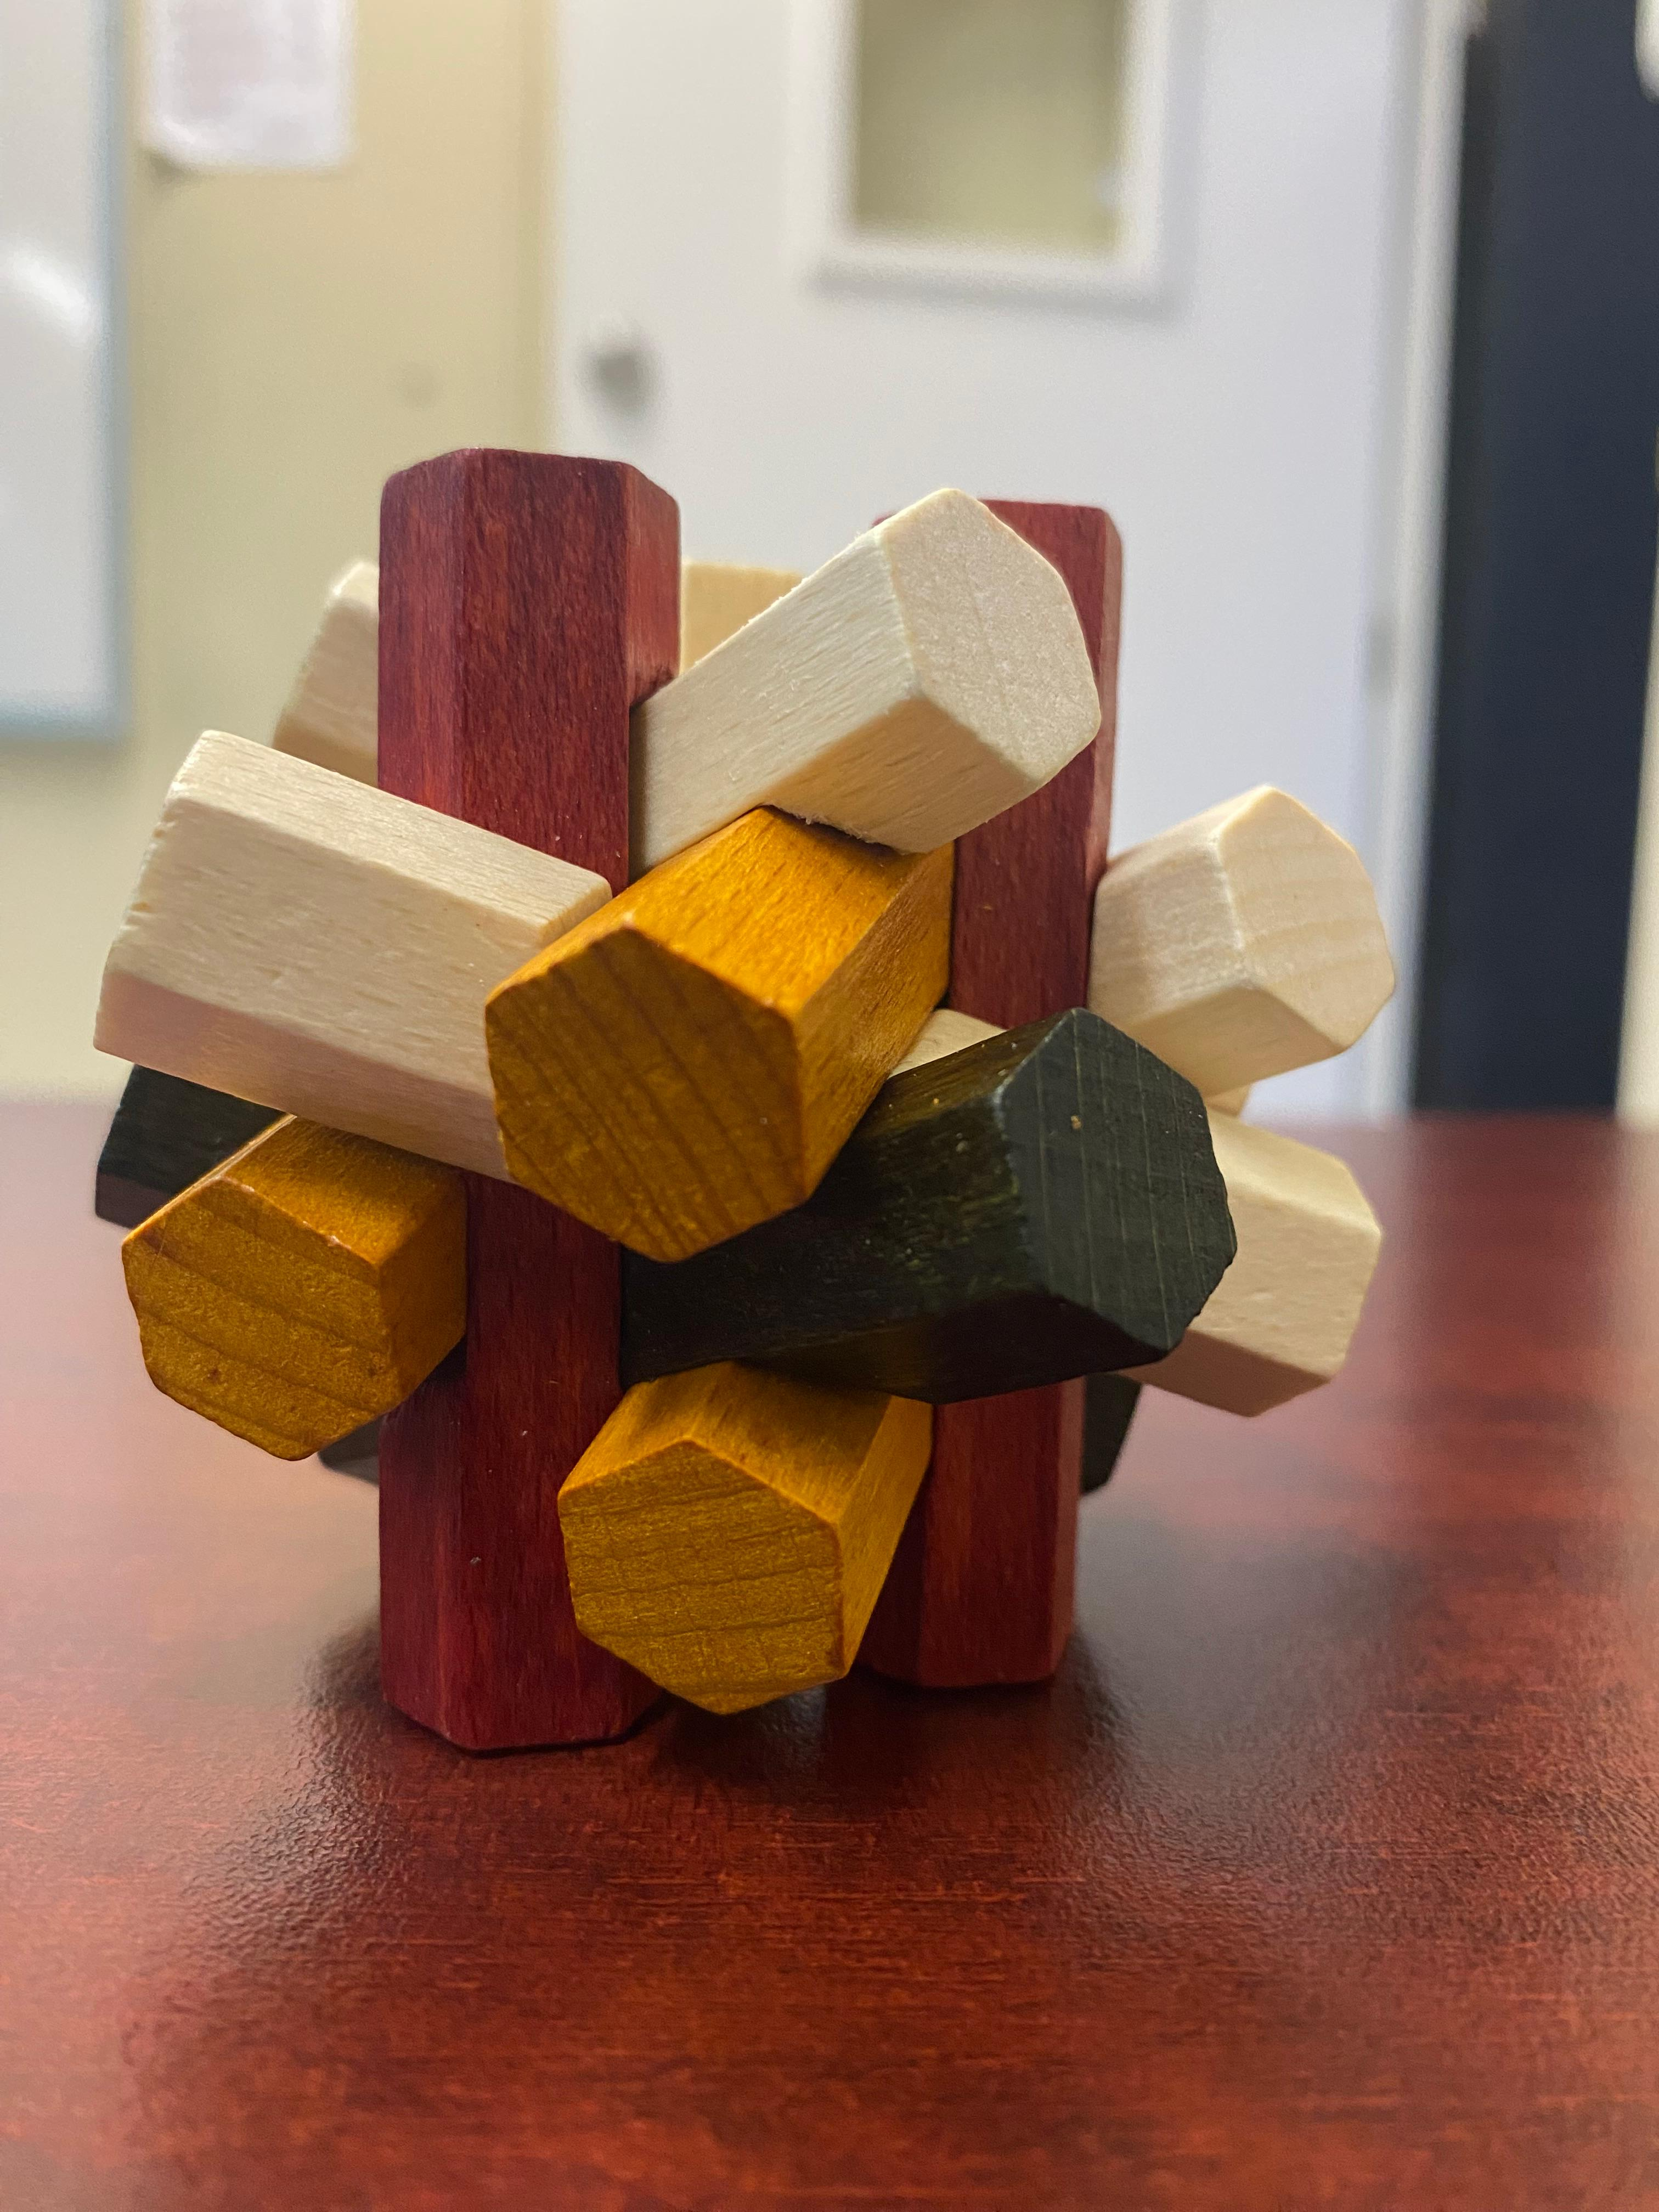
\includegraphics[scale = 0.04]{clases/images/clase7/R1-1.jpeg}&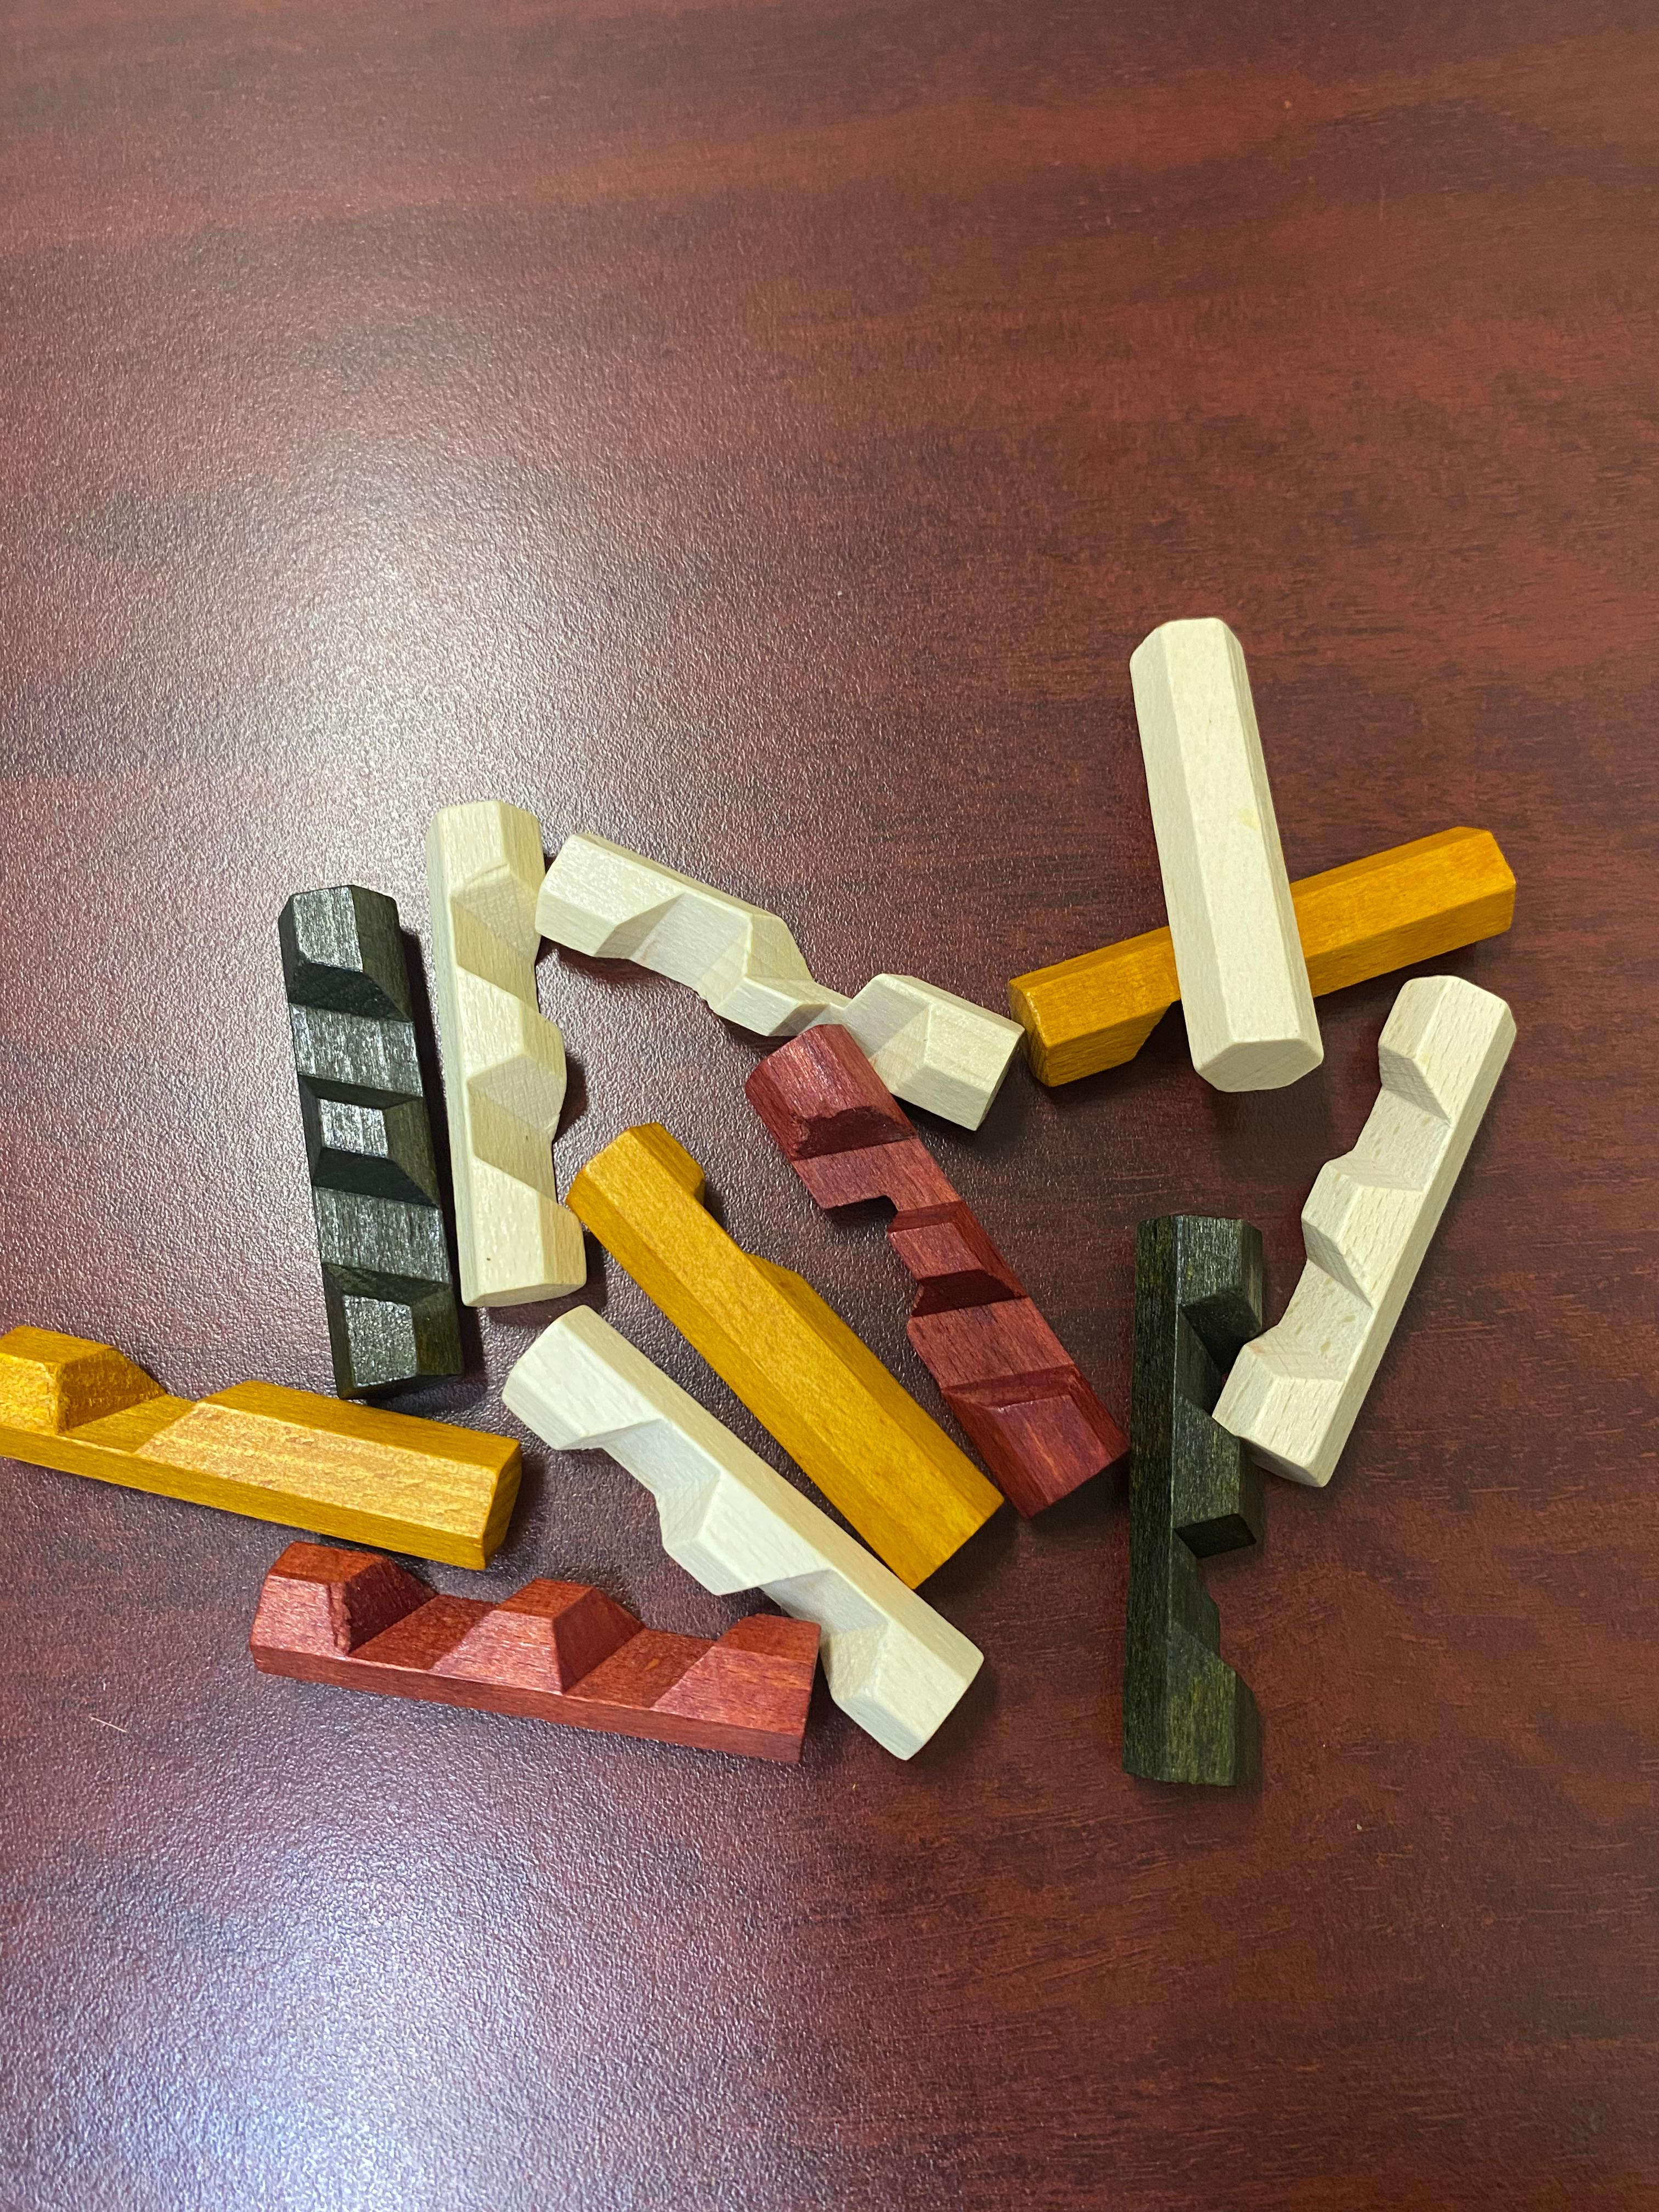
\includegraphics[scale = 0.04]{clases/images/clase7/R1-2.jpeg}
    \end{tabular}
    \caption{}
\end{figure}

Debido a que en el primer problema me llevé alrededor de una hora y 15 minutos, sólo pude armar tres rompecabezas más

\section{Rompecabezas 2}

Sin desensamblar el cubo lo fui observando, moviendo cada pieza ligeramente para intentar ver cómo se conectaban. Luego lo deshice para comenzar con el proceso de armado y por mis observaciones, las piezas que iban en las esquinas del cubo tenían forma de L y a partir de ahí solo fui haciendo permutaciones respecto a la posición de cada pieza.

\begin{figure}[H]
    \begin{tabular}{ccc}
        Inico & Proceso & Final\\\\
        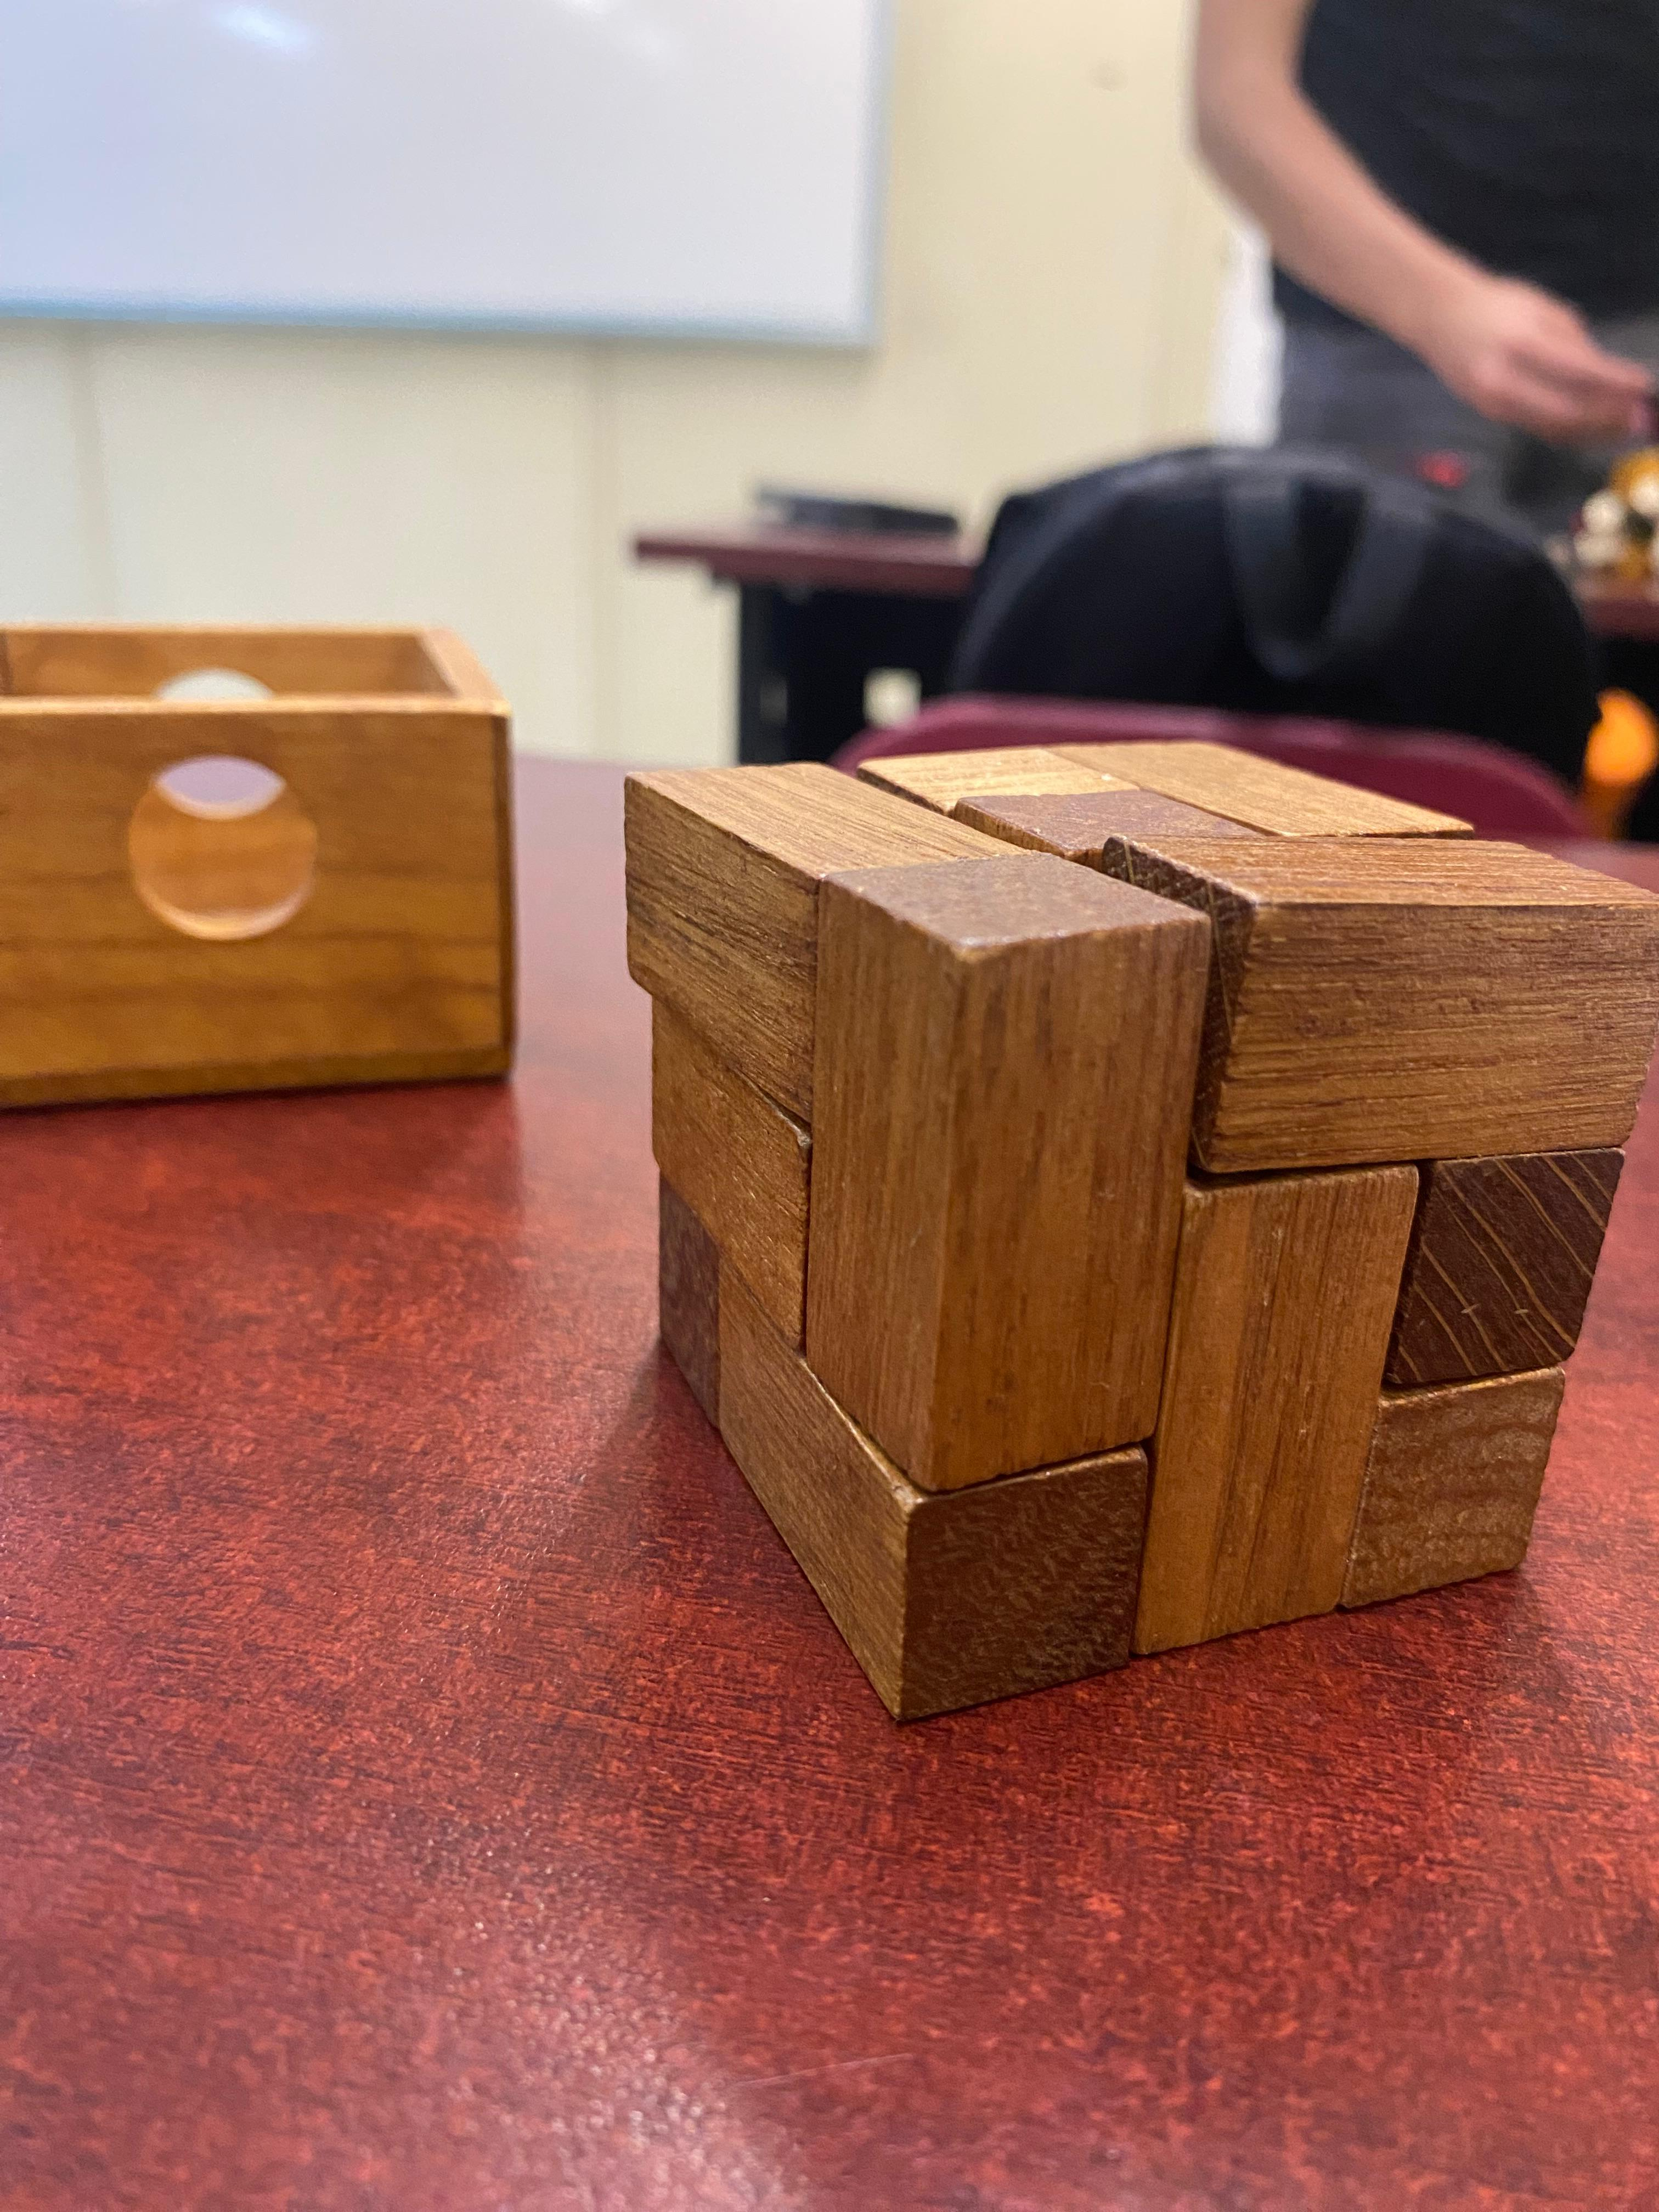
\includegraphics[scale = 0.04]{clases/images/clase7/R2Inicio.jpeg}&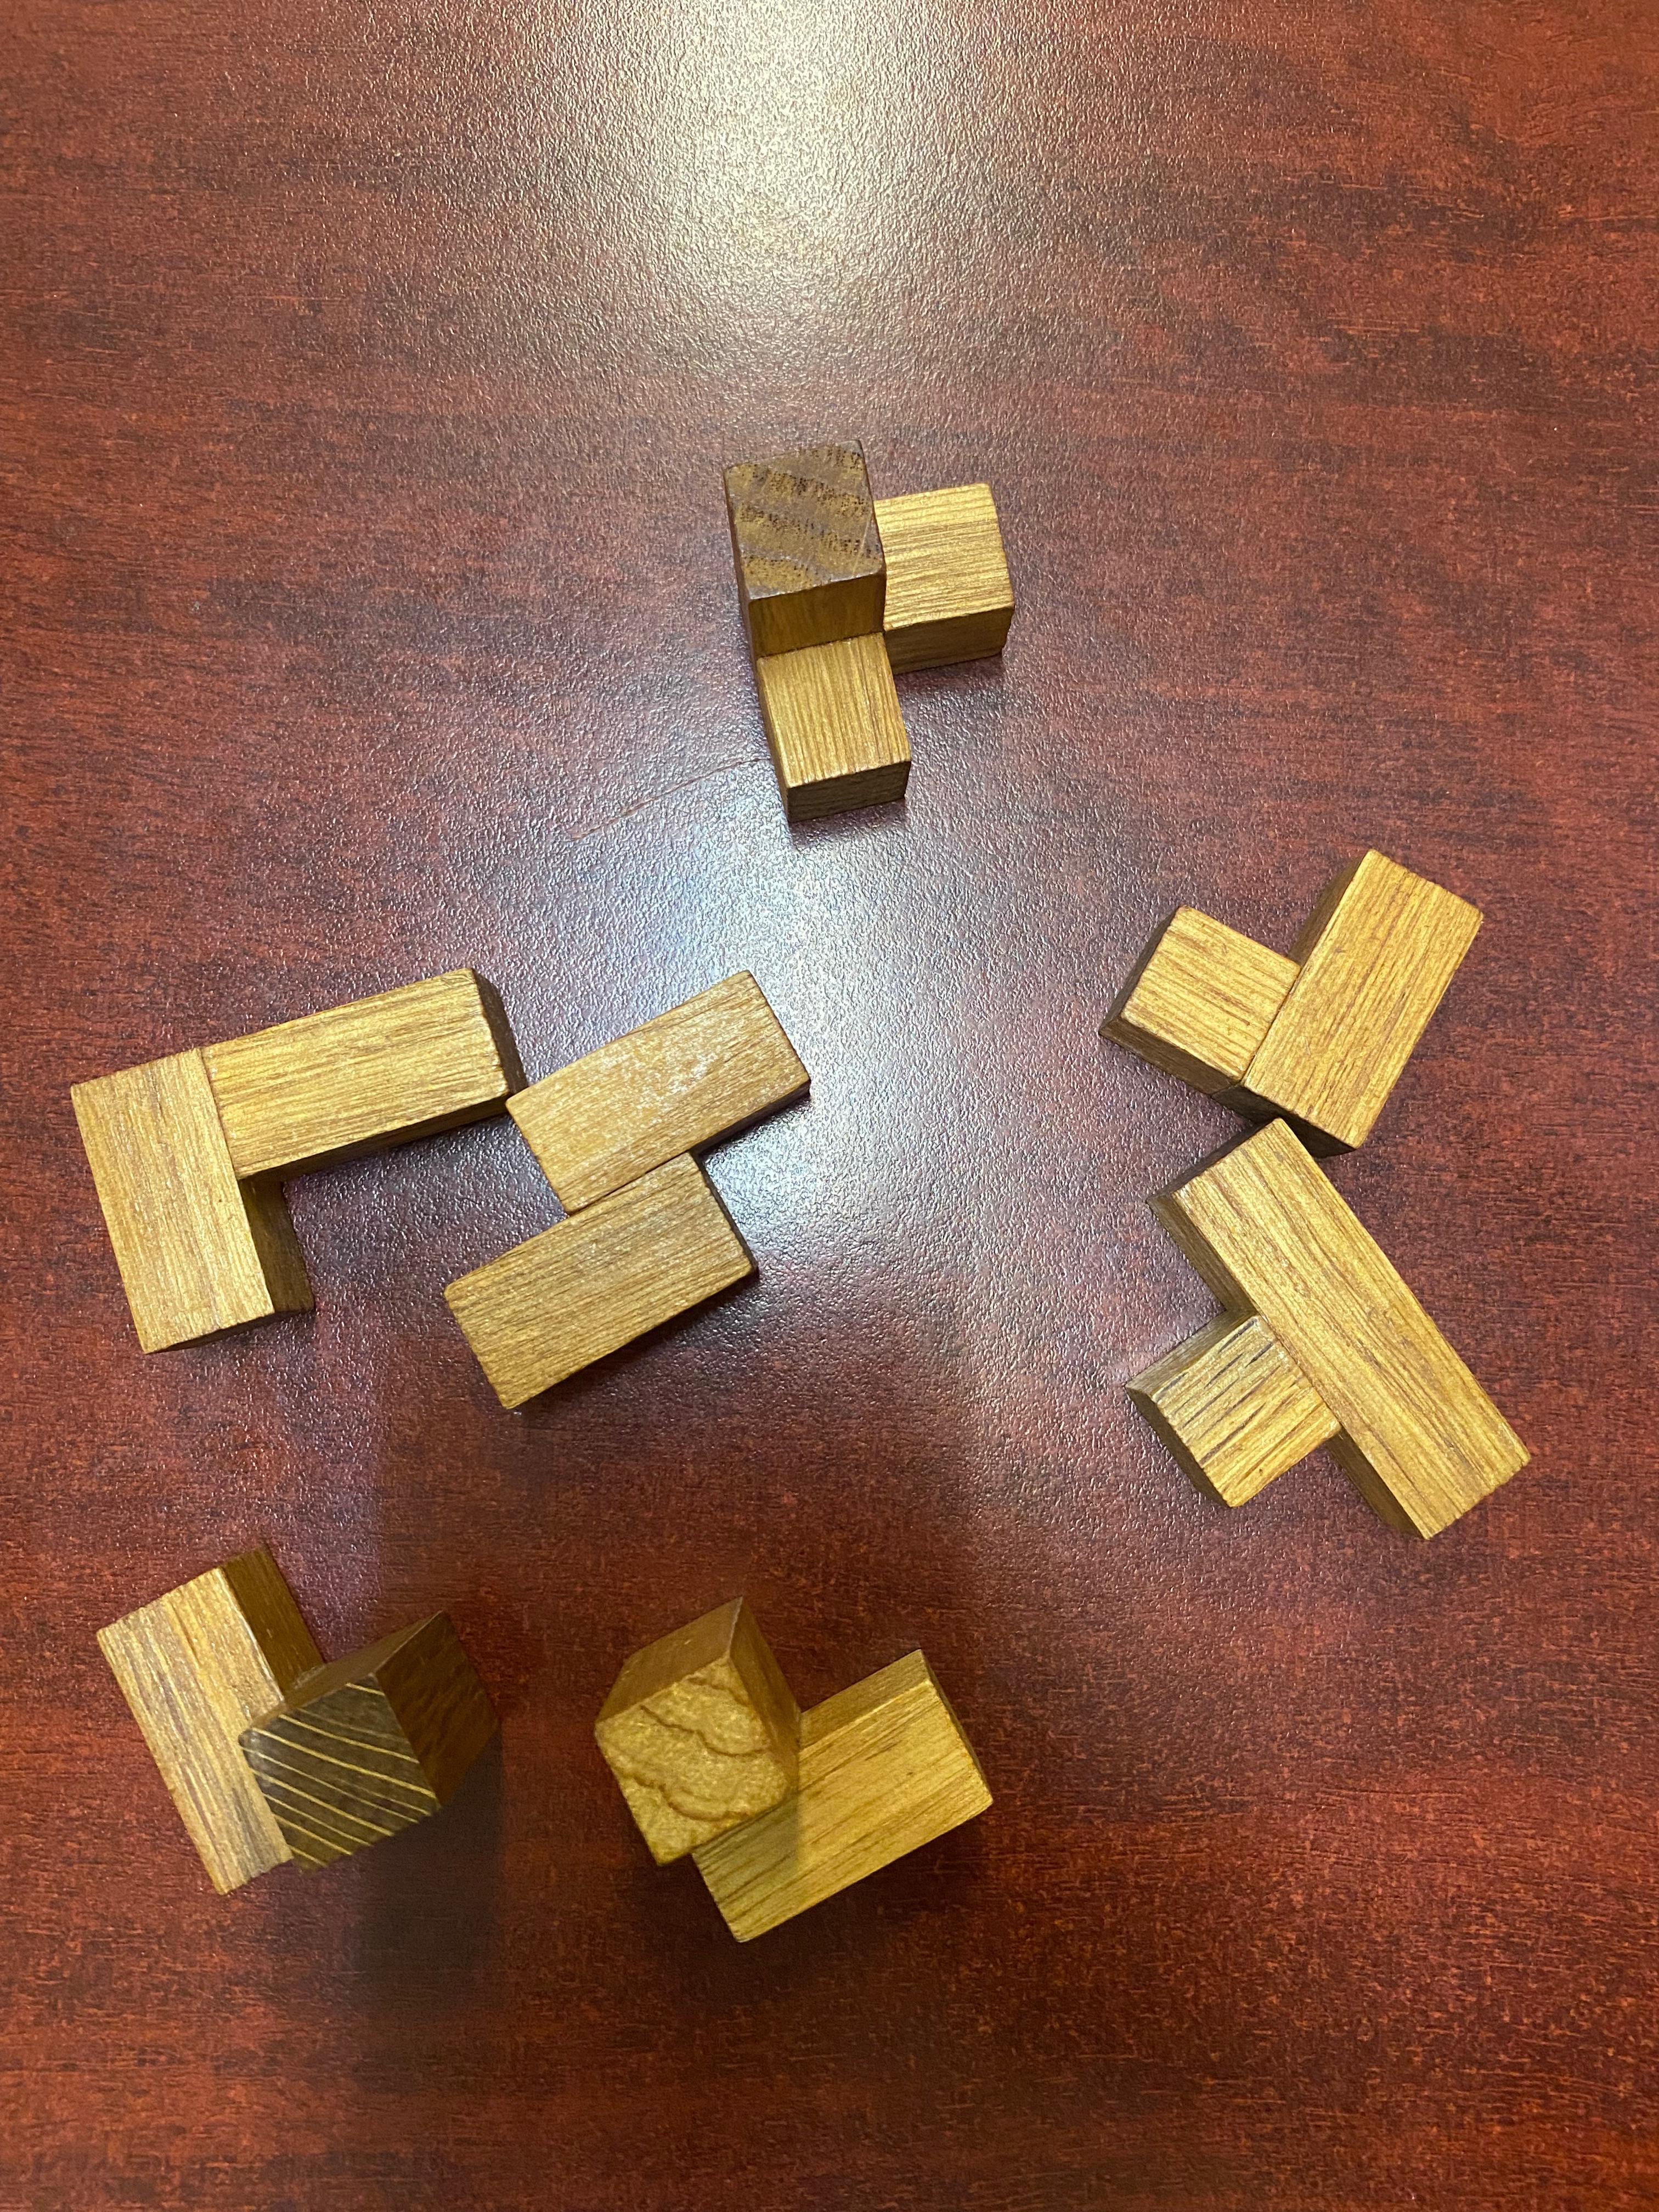
\includegraphics[scale = 0.04]{clases/images/clase7/R2Proceso.jpeg}&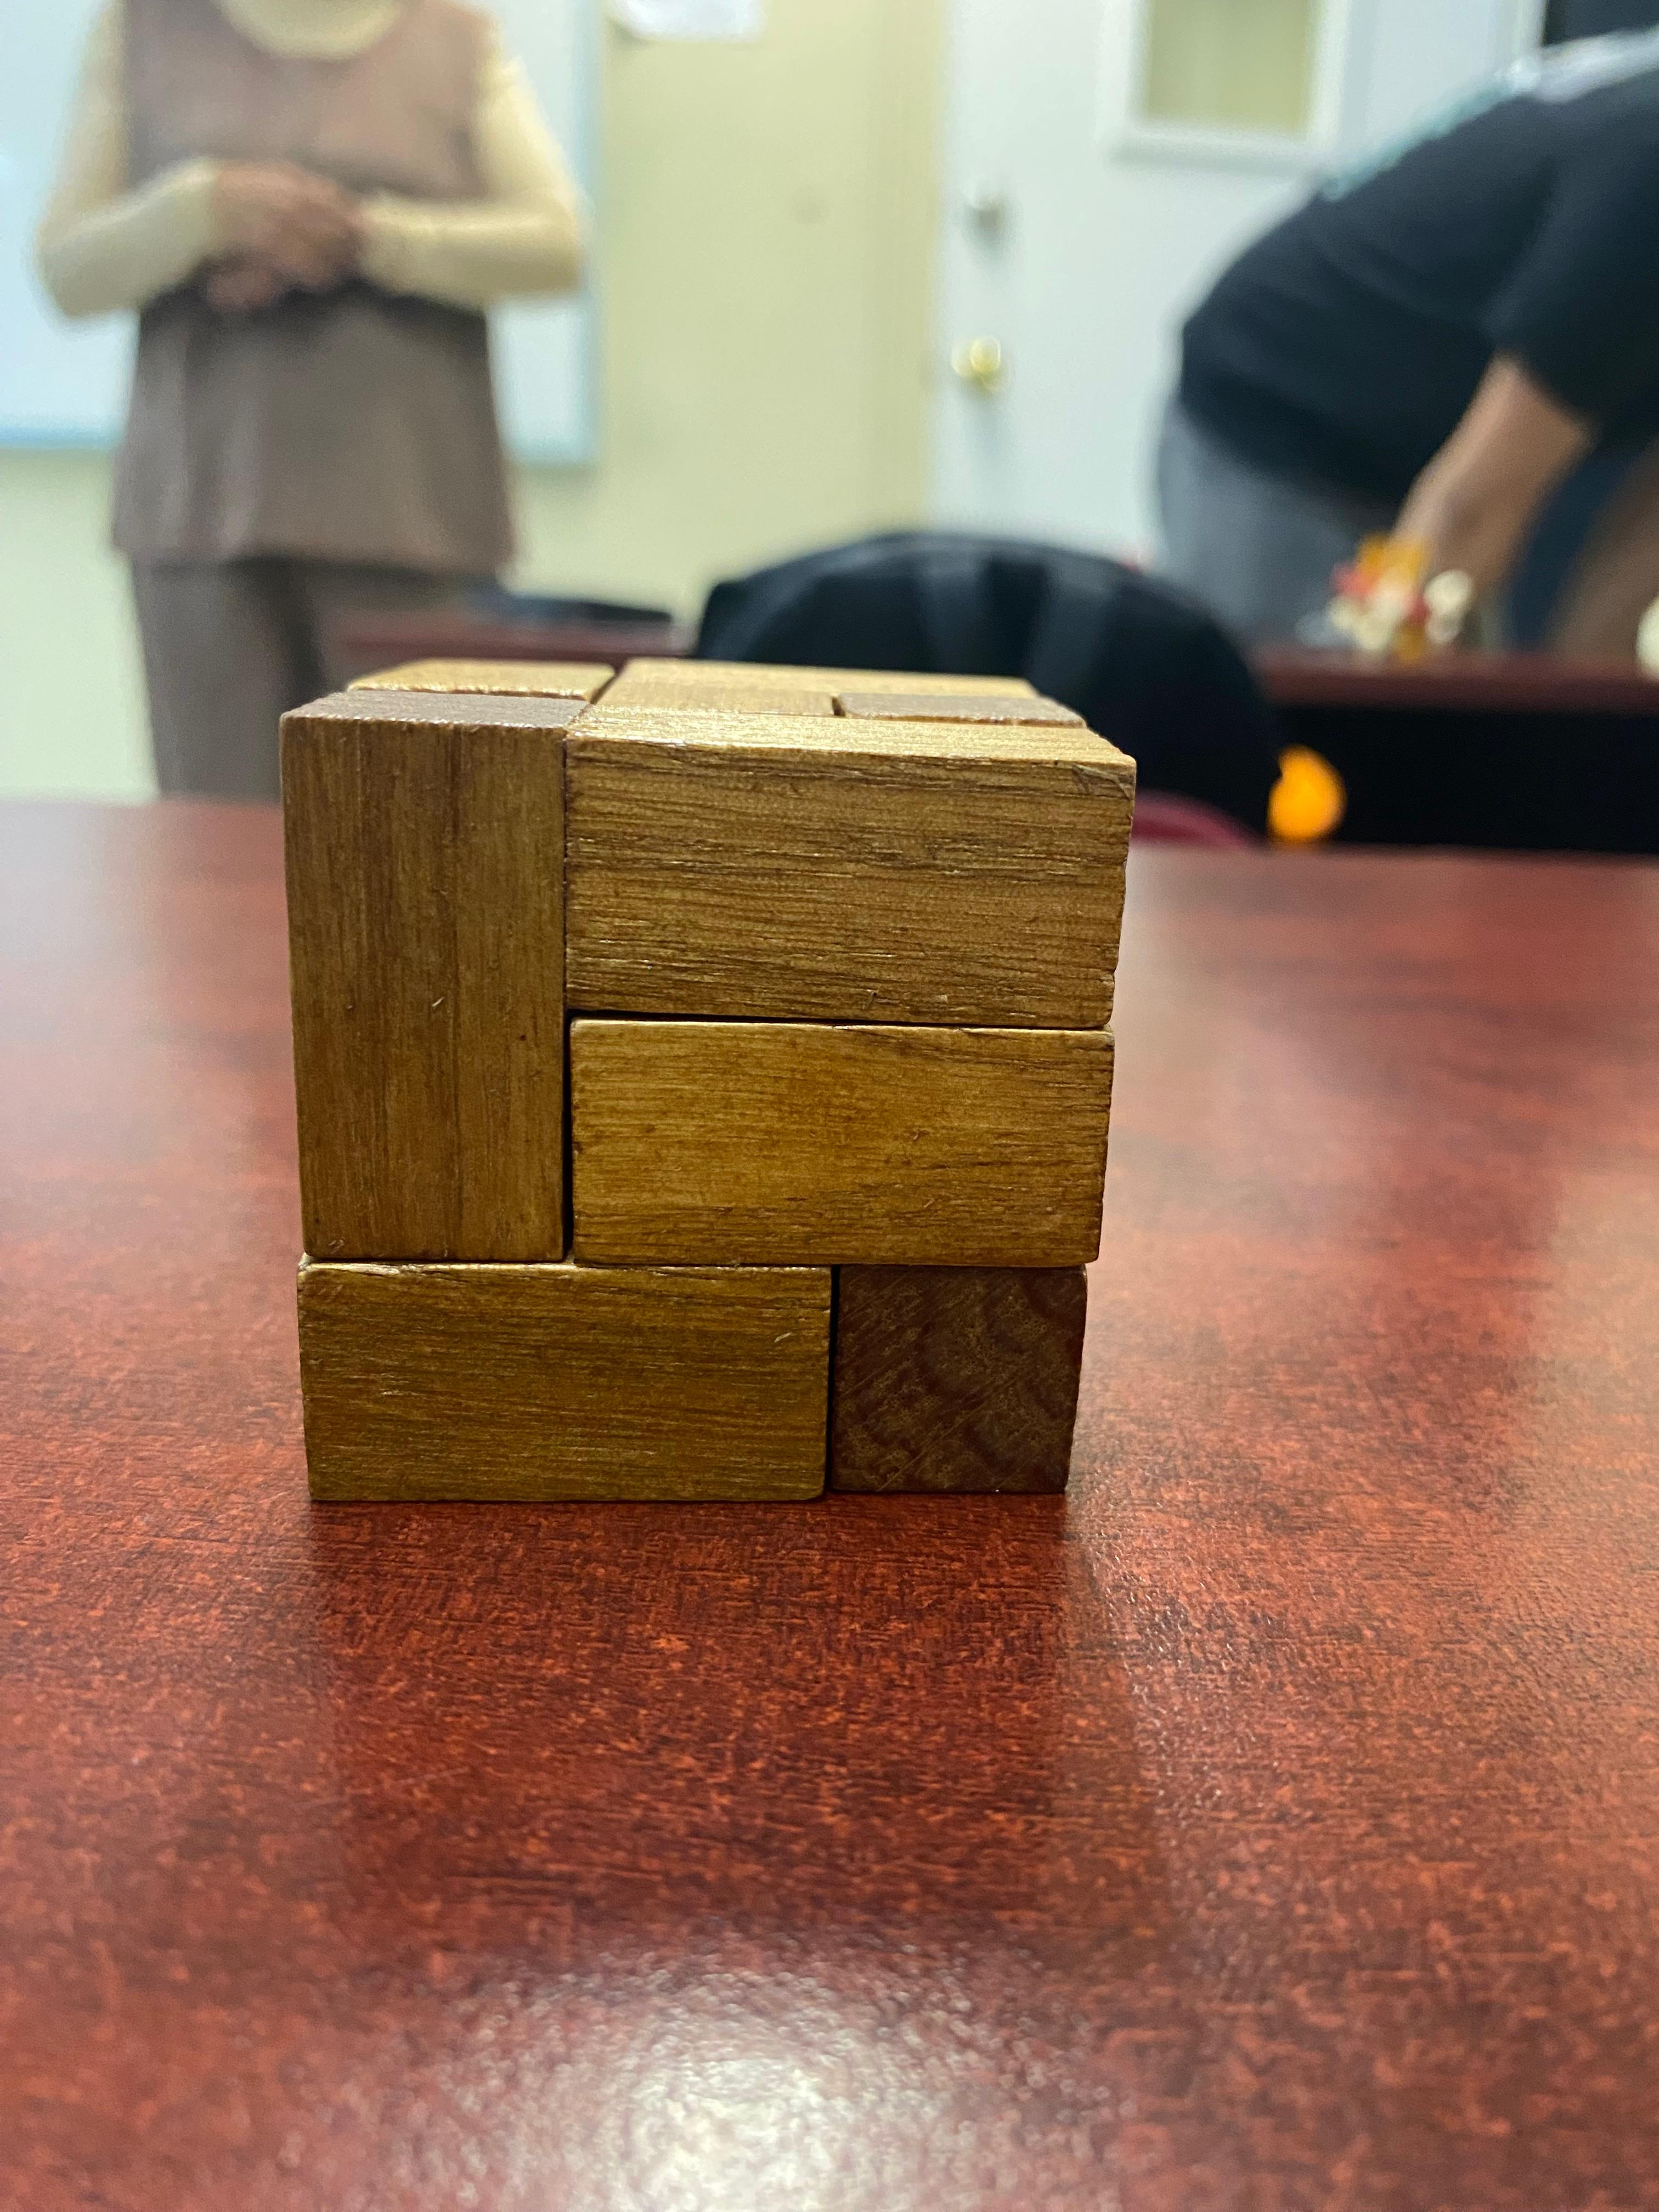
\includegraphics[scale = 0.04]{clases/images/clase7/R2Final.jpeg}
    \end{tabular}
    \caption{}
\end{figure}

\section{Rompecabezas 3}

Este rompecabezas iniciaba con cuatro T las cuales debía acomodar dentro del tablero sin que se salieran ni se amontonaran; Las primeras dos soluciones no me costaron tanto como la tercera.

\begin{figure}[H]
    \begin{tabular}{ccc}
        \multicolumn{3}{c}{SOLUCIONES}\\
        1 & 2 & 3\\\\
        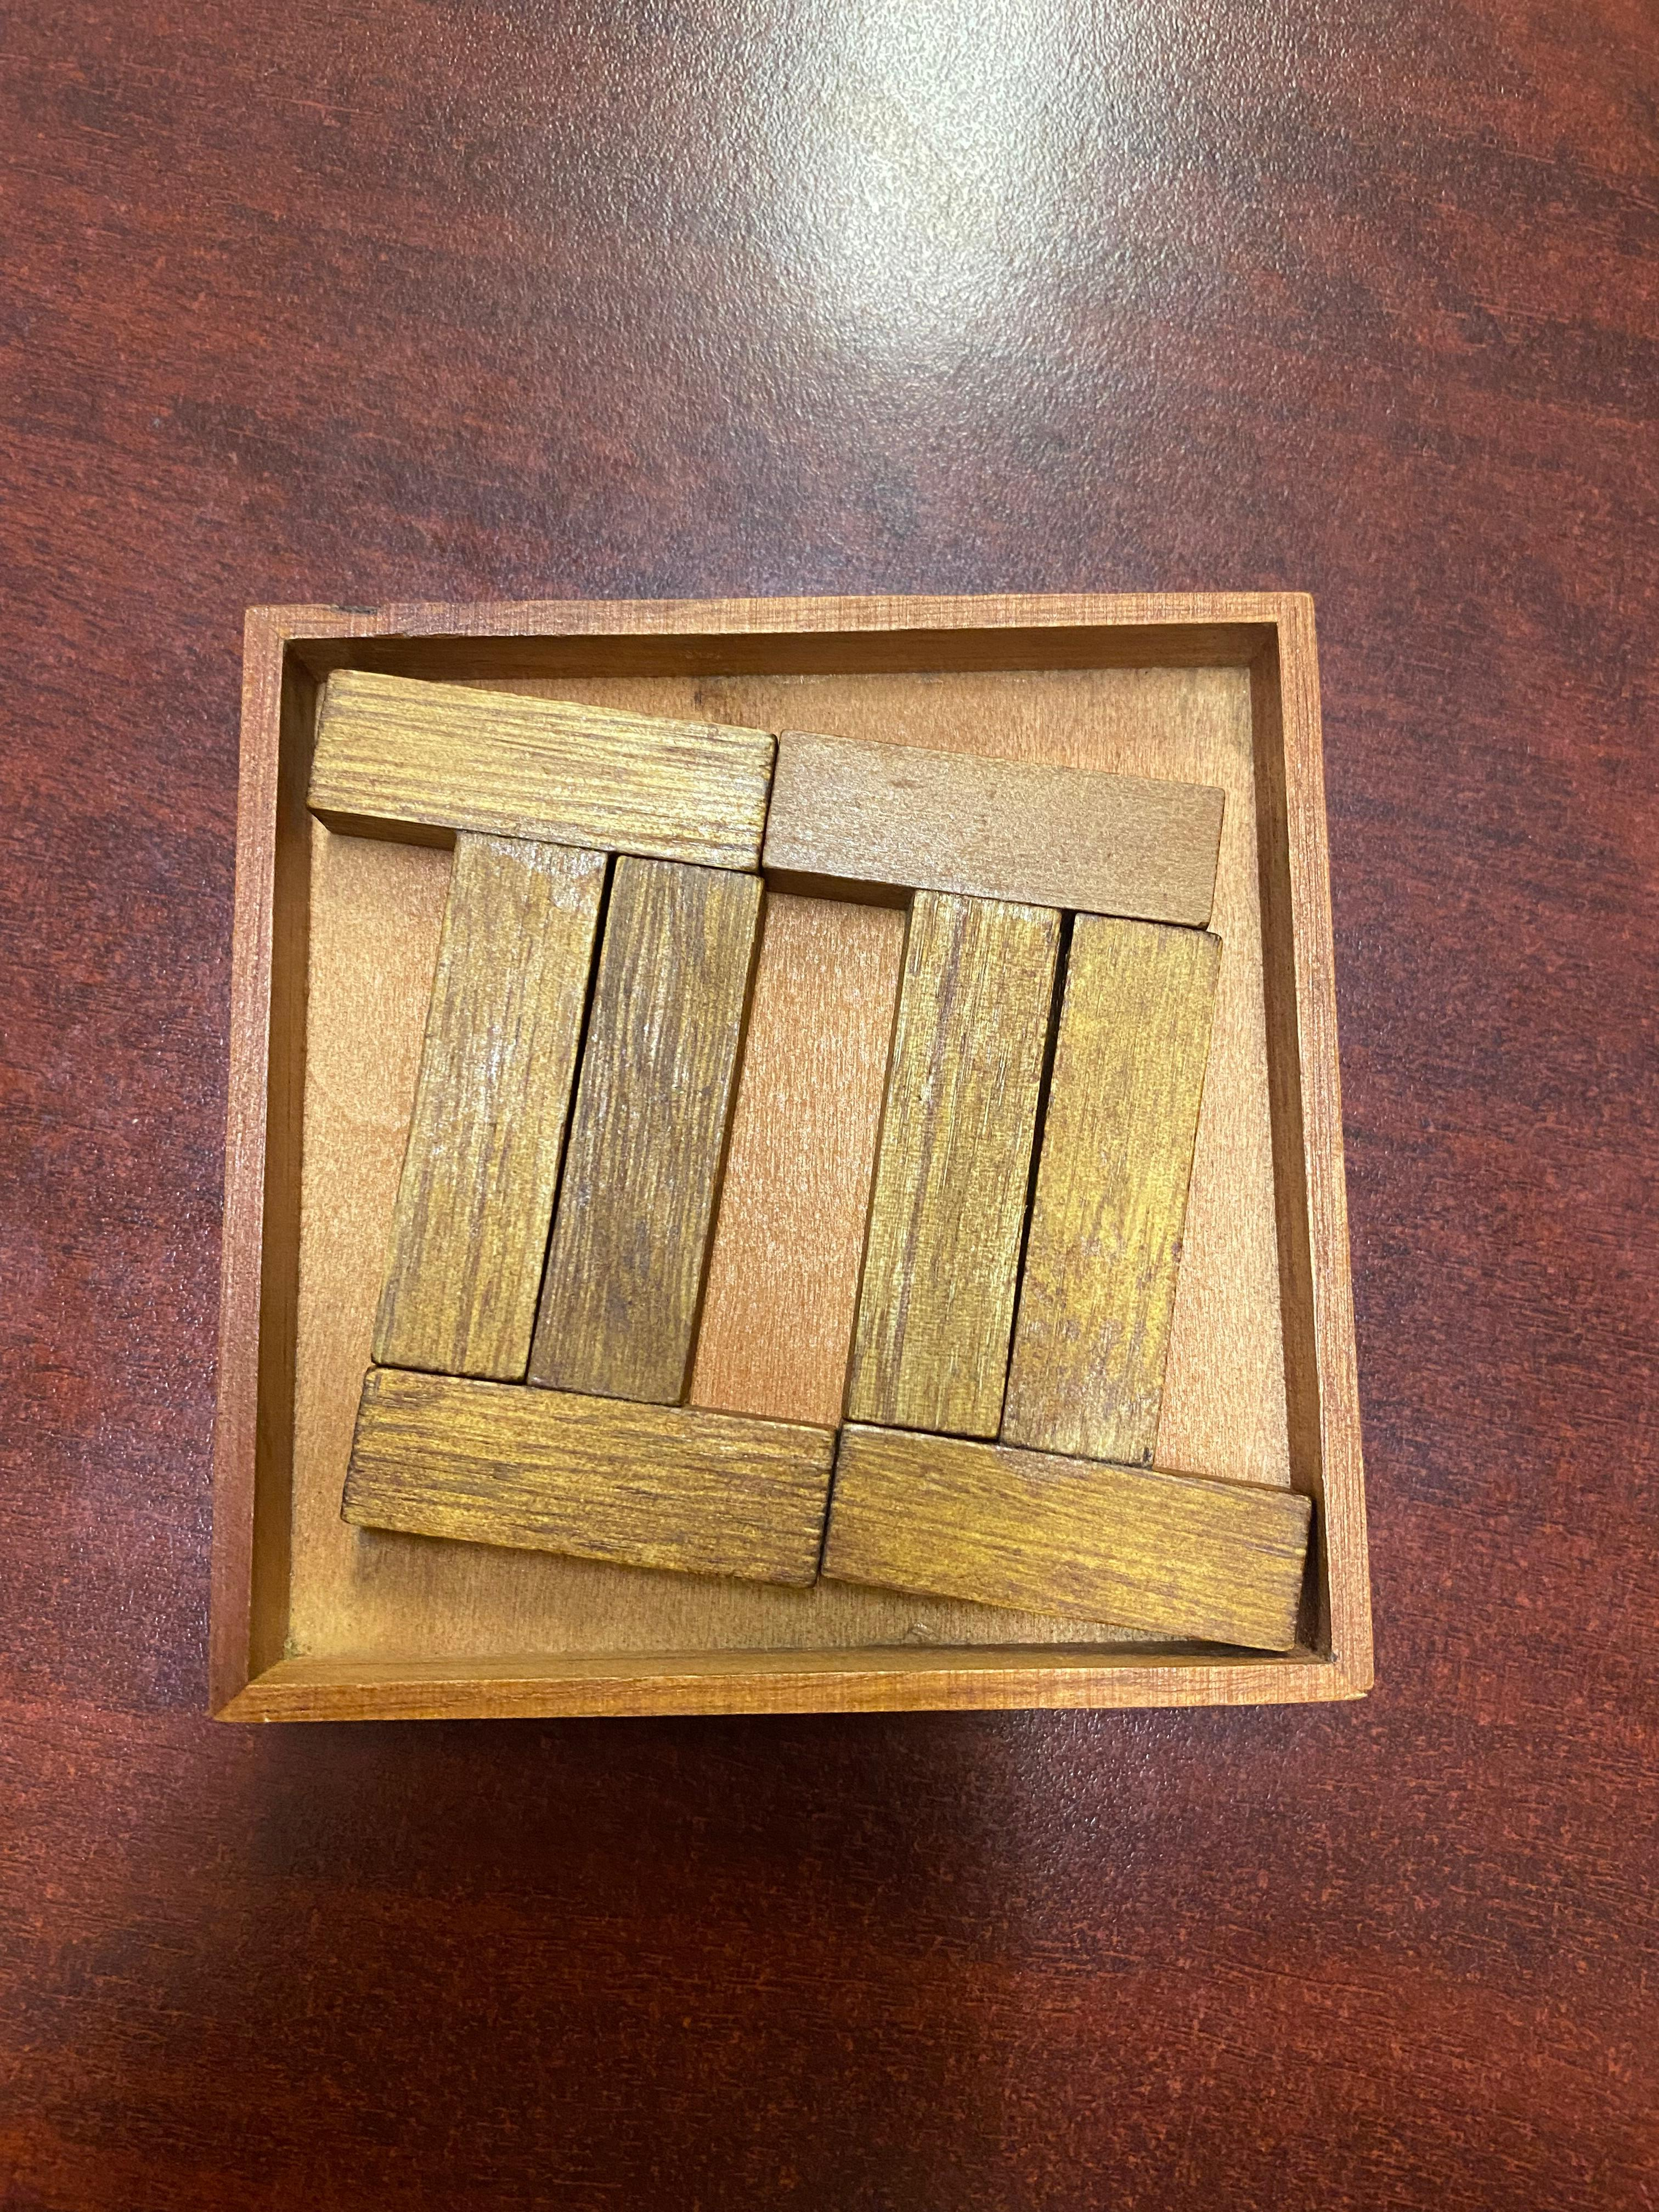
\includegraphics[scale = 0.04]{clases/images/clase7/R3-Sol1.jpeg}&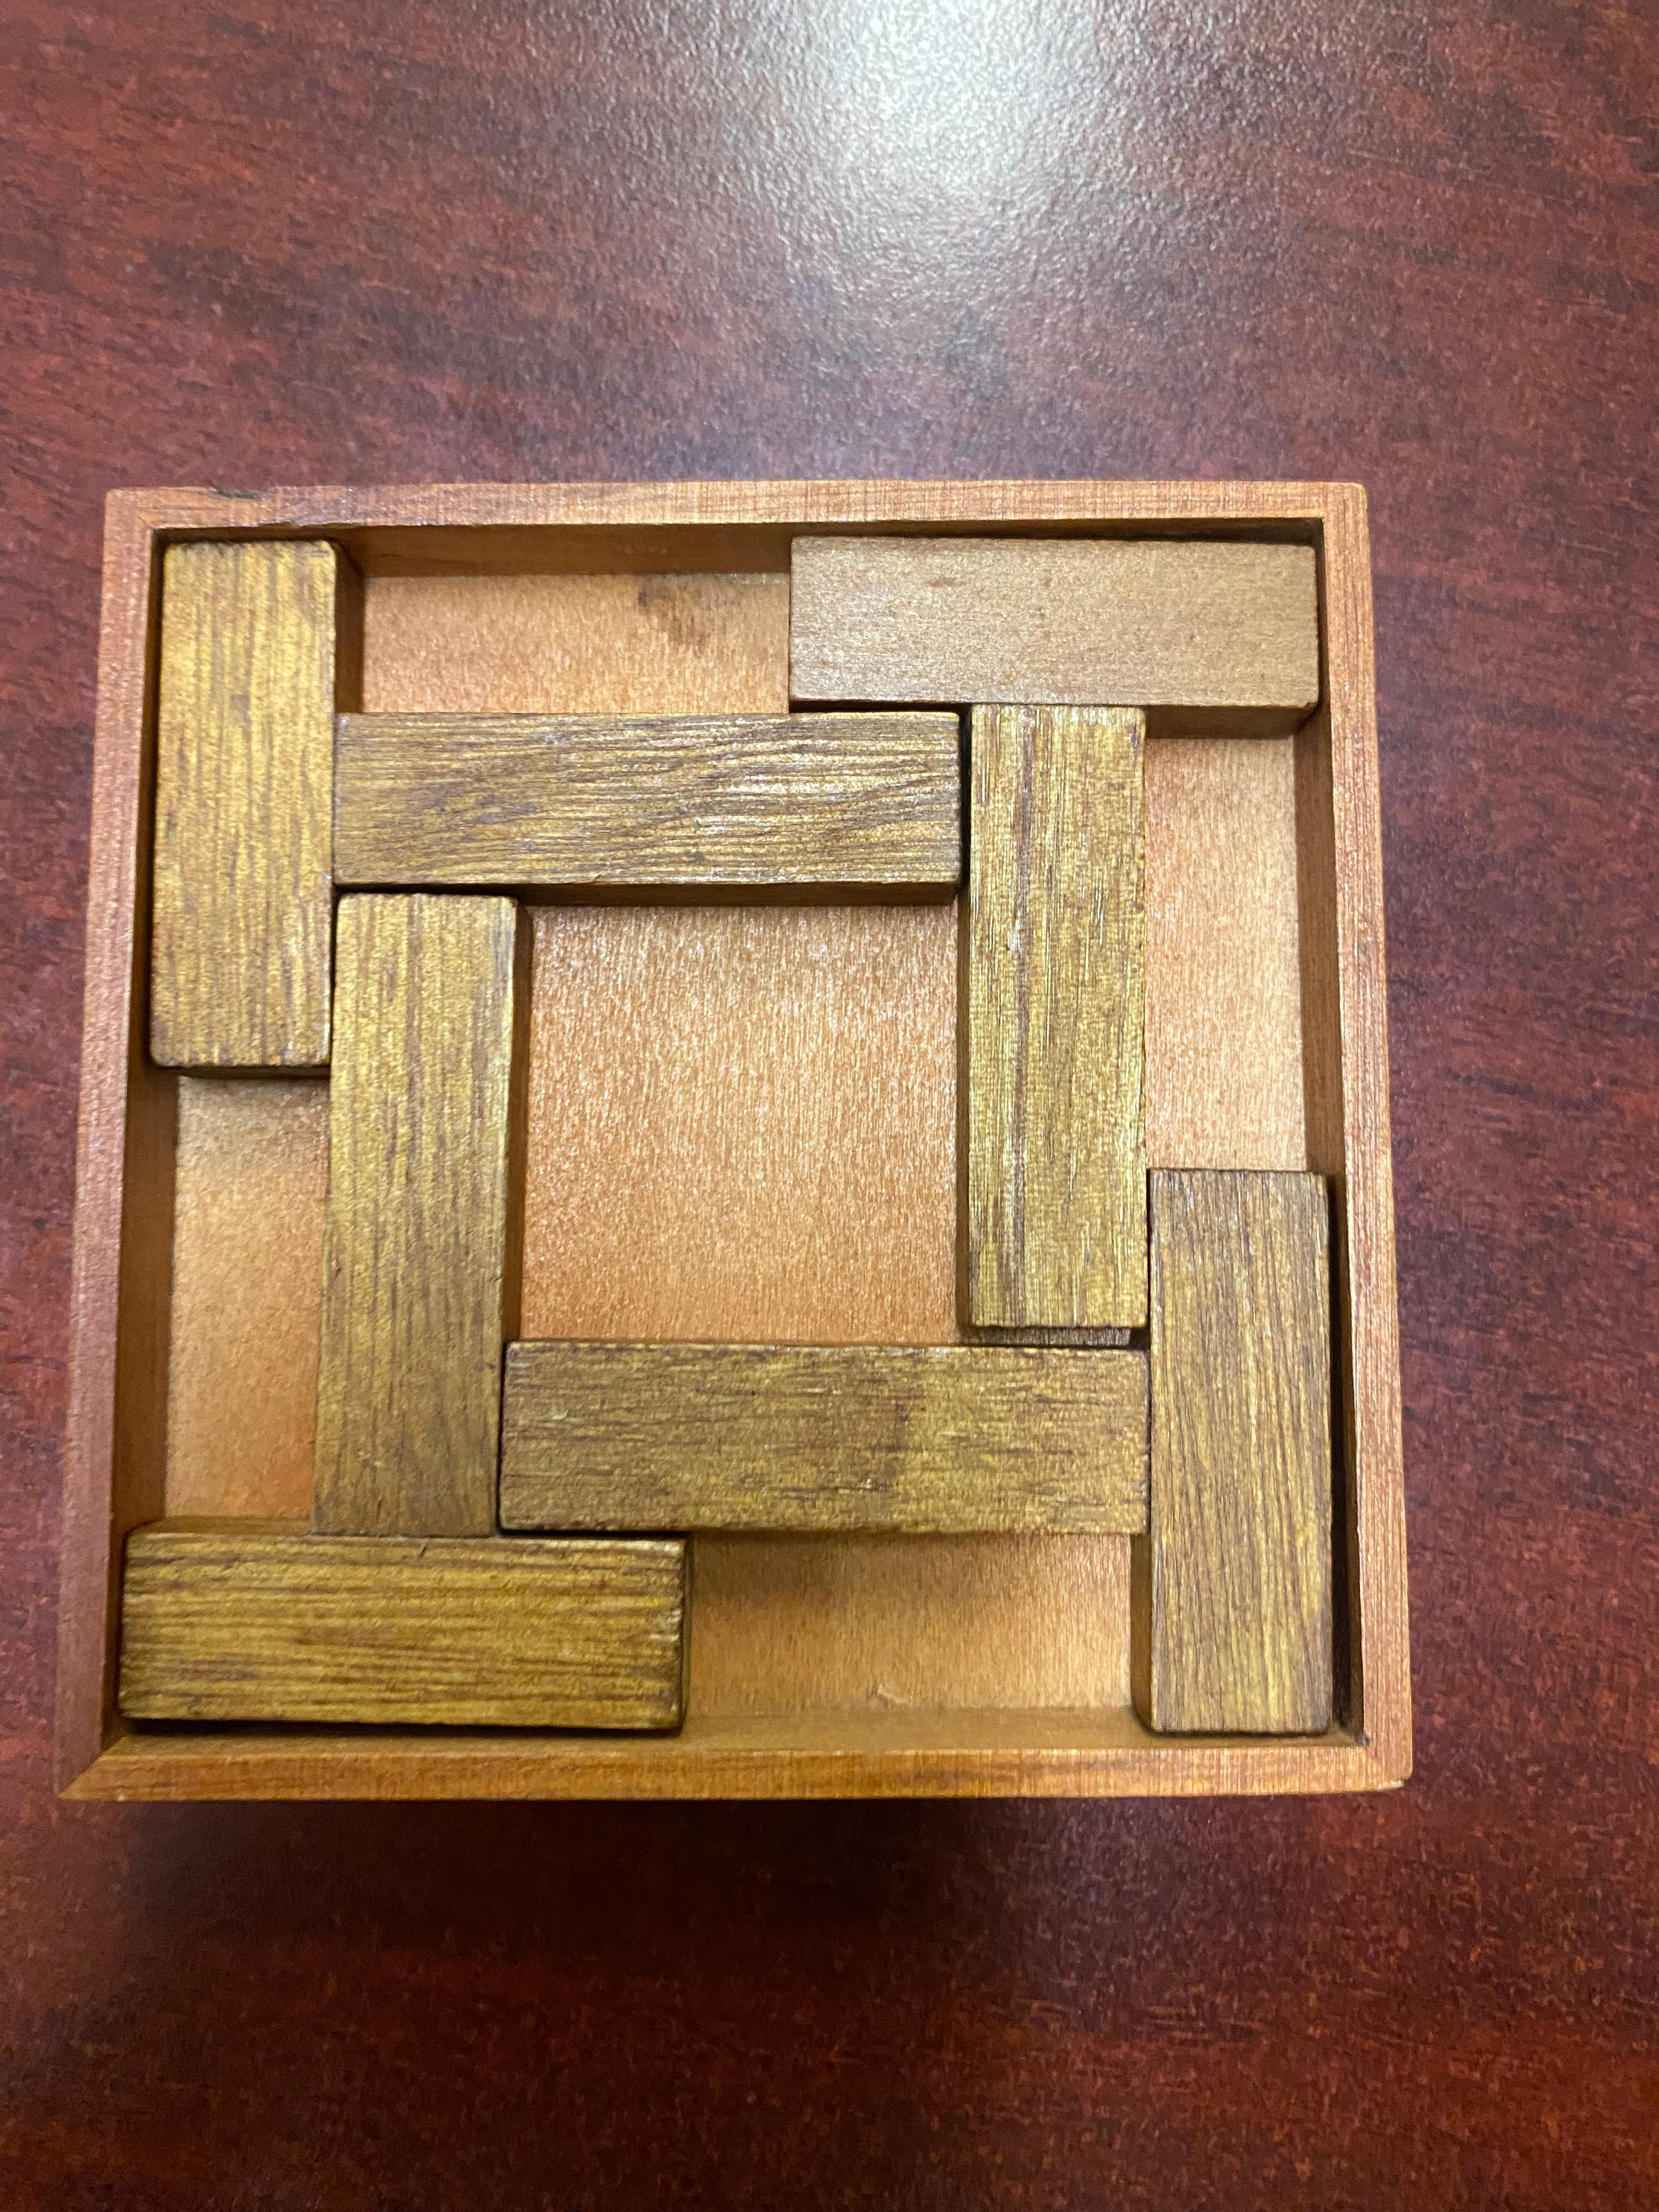
\includegraphics[scale = 0.04]{clases/images/clase7/R3-Sol2.jpeg}&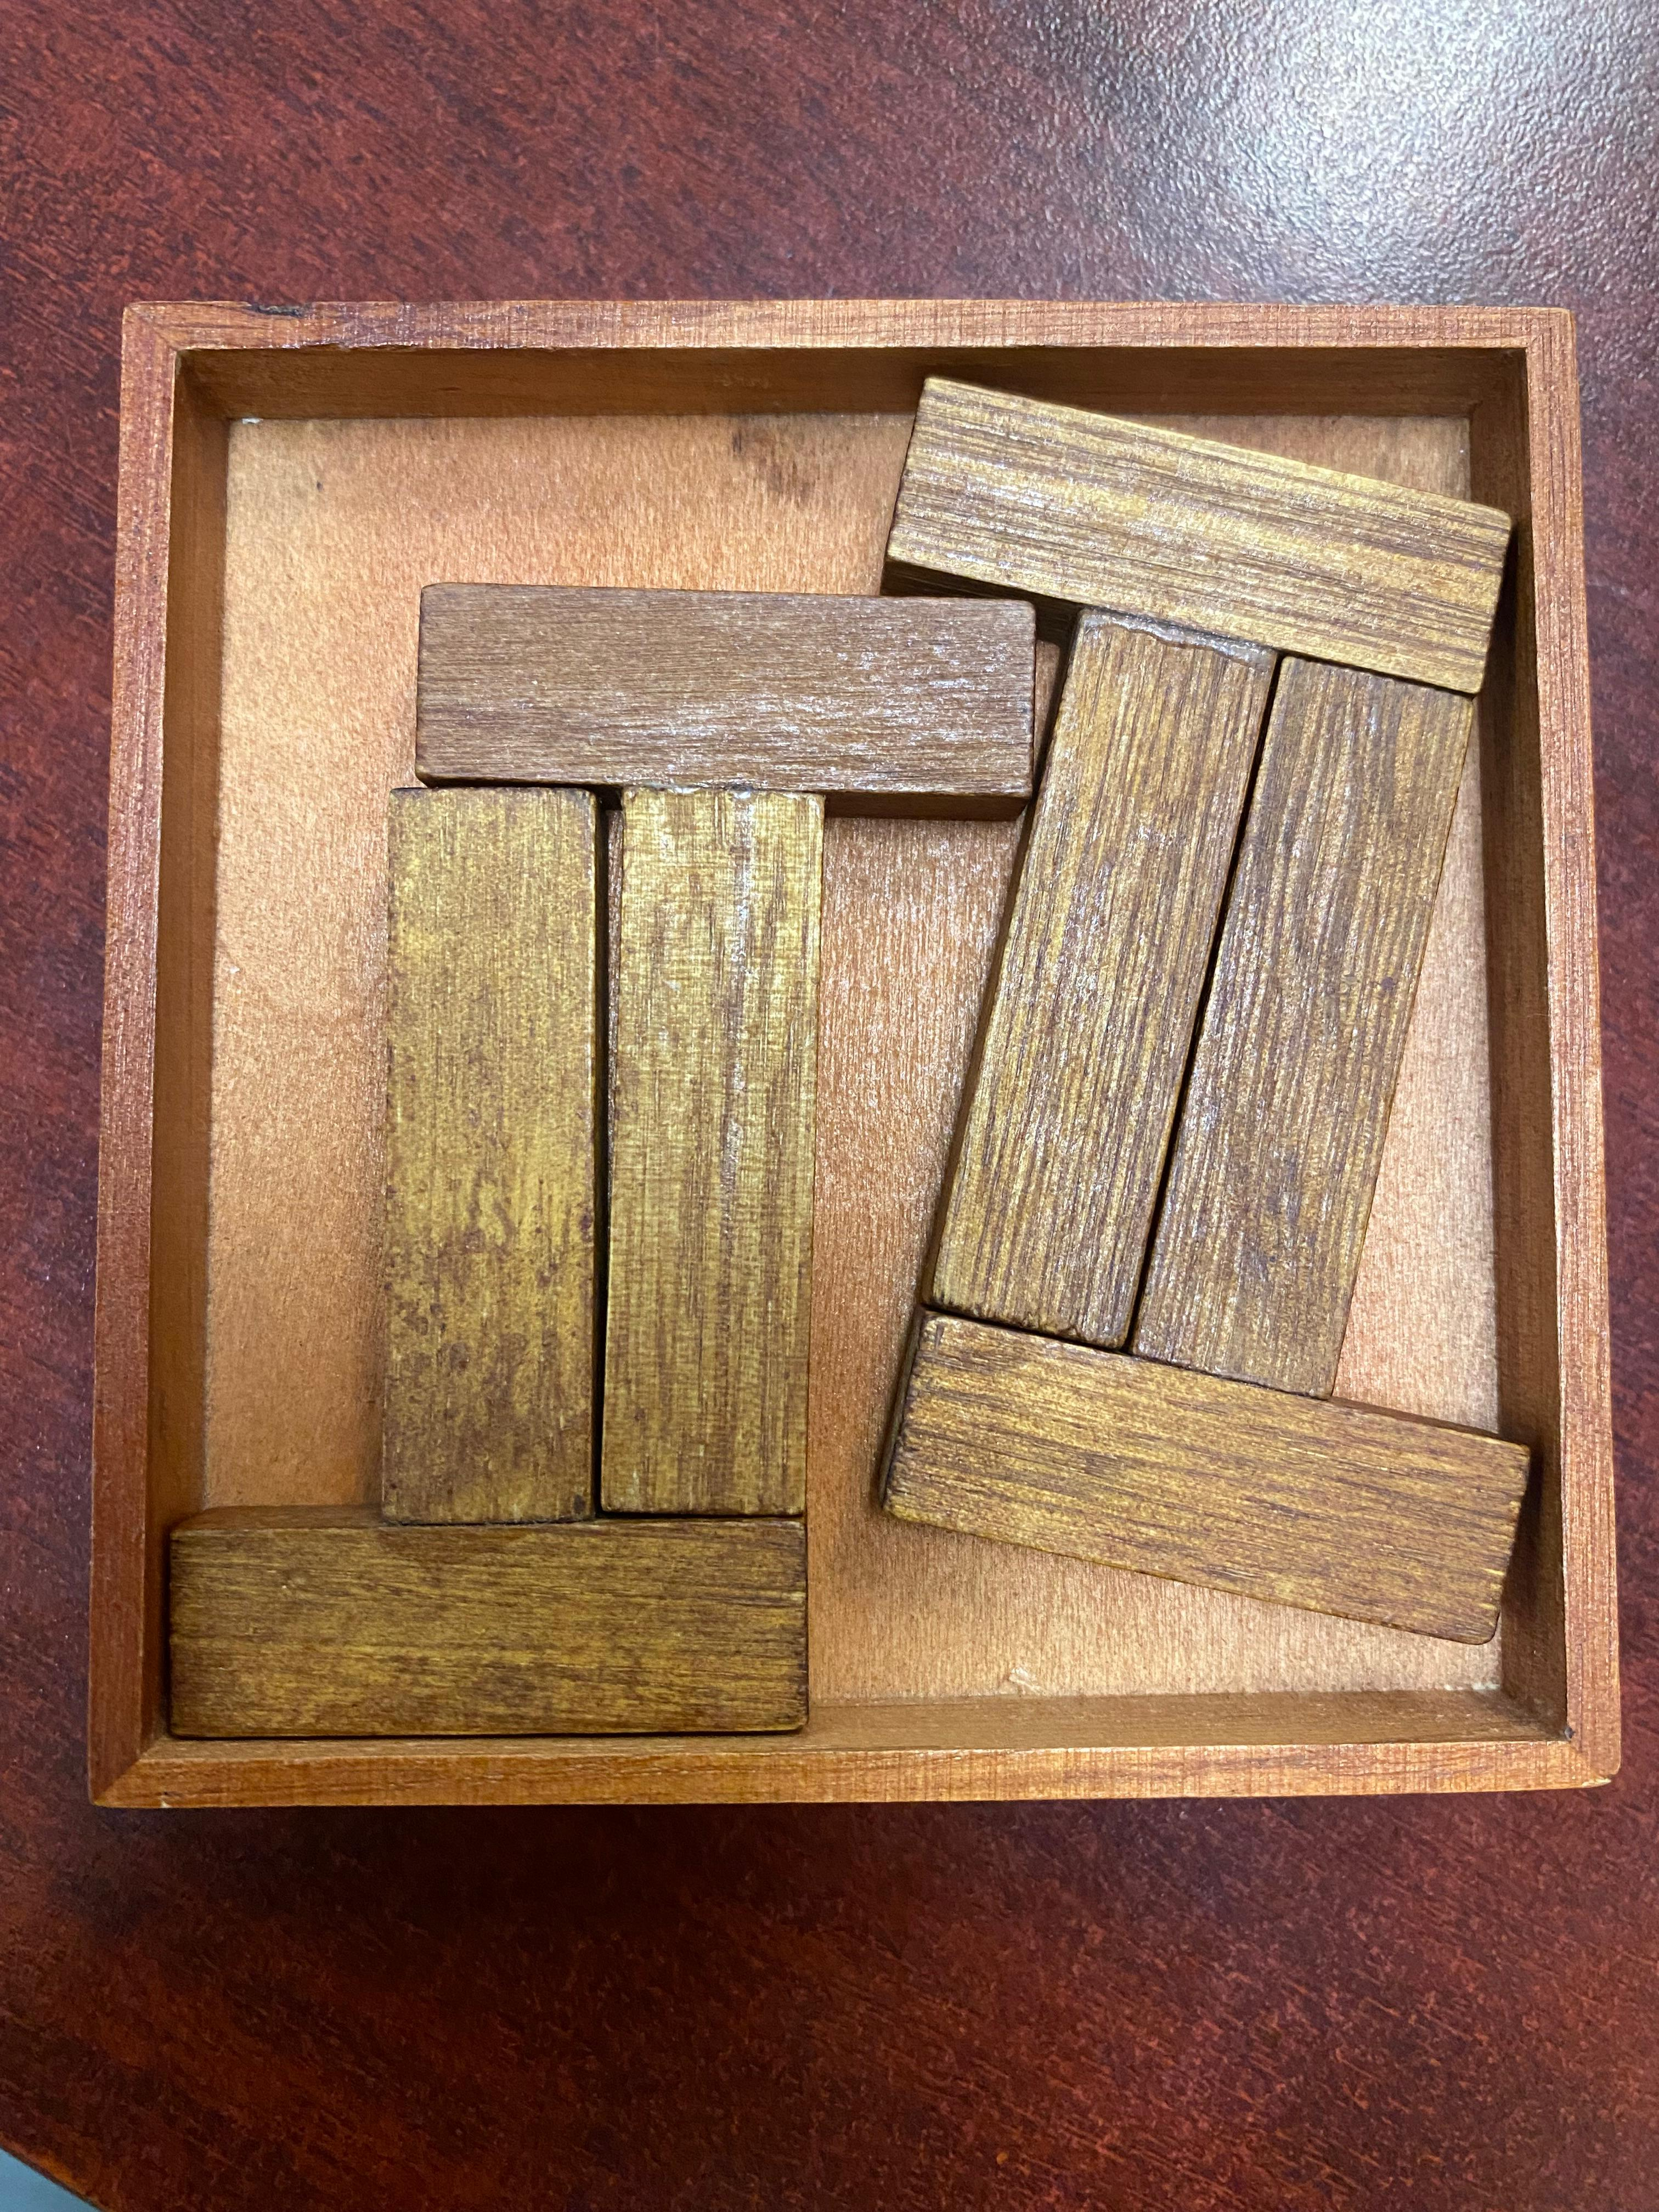
\includegraphics[scale = 0.04]{clases/images/clase7/R3-Sol3.jpeg}
    \end{tabular}
    \caption{}
\end{figure}